\section{Proposed Method}
Existing specification-based malware detectors can be utilized if we extract
the correlation between shadow processes efficiently, because with that correlation
we are able to reconstruct the original system call graph from system call sequences
of shadow processes. In this section, we propose the design of a system method to extract the correlation.

\subsection{Problem Scope}
We focus on only shadow attacks that performs Inter-Process Communication, or IPC, via unix domain socket.

\cite{Weiqin:ShadowAttack} showed prototype implementation of a compiler
that takes existing malware as input and outputs the executable of malware of shadow-attack version.
Therefore, it is reasonable to infer that shadow attacks based on IPC through unix domain socket
are highly feasible, and they should be considered as a significant threat.

\subsection{Key Concepts (tentative)}
As mentioned before, shadow attacks are the strategy where malware exports its critical system calls
to shadow processes and hyde its malicious behavior.
\cite{Weiqin:ShadowAttack} listed examples of system calls that are critical for malware's intent,
shown in \Tref{tab:critical-system-calls}.

Among these system calls, file-related and network-related system calls handle file descriptors:
\texttt{open} and \texttt{socket} create a new file descriptor,
while others access the file tied to the file descriptor or perform network communication.
So shadow processes need to transfer file descriptors to each other to perform the file-related and
network-related system calls. This concept is shown in \Fref{img:fd-transfer}.

\begin{table*}[t]
  \caption{Examples of critical system calls. This table is reconstructed by the author from \cite{Weiqin:ShadowAttack}.}
  \centering
  \begin{tabular}{|l|l|}
    \hline
    \textbf{Function Category} & \textbf{System Call}                     \\
    \hline
    File I/O operation         & open, read, write                        \\
    \hline
    Network                    & socket, connect, recv, send, read, write \\
    \hline
    Process management         & exec, execl                              \\
    \hline
  \end{tabular}
  \label{tab:critical-system-calls}
\end{table*}

\begin{figure*}[t]
  \begin{center}
    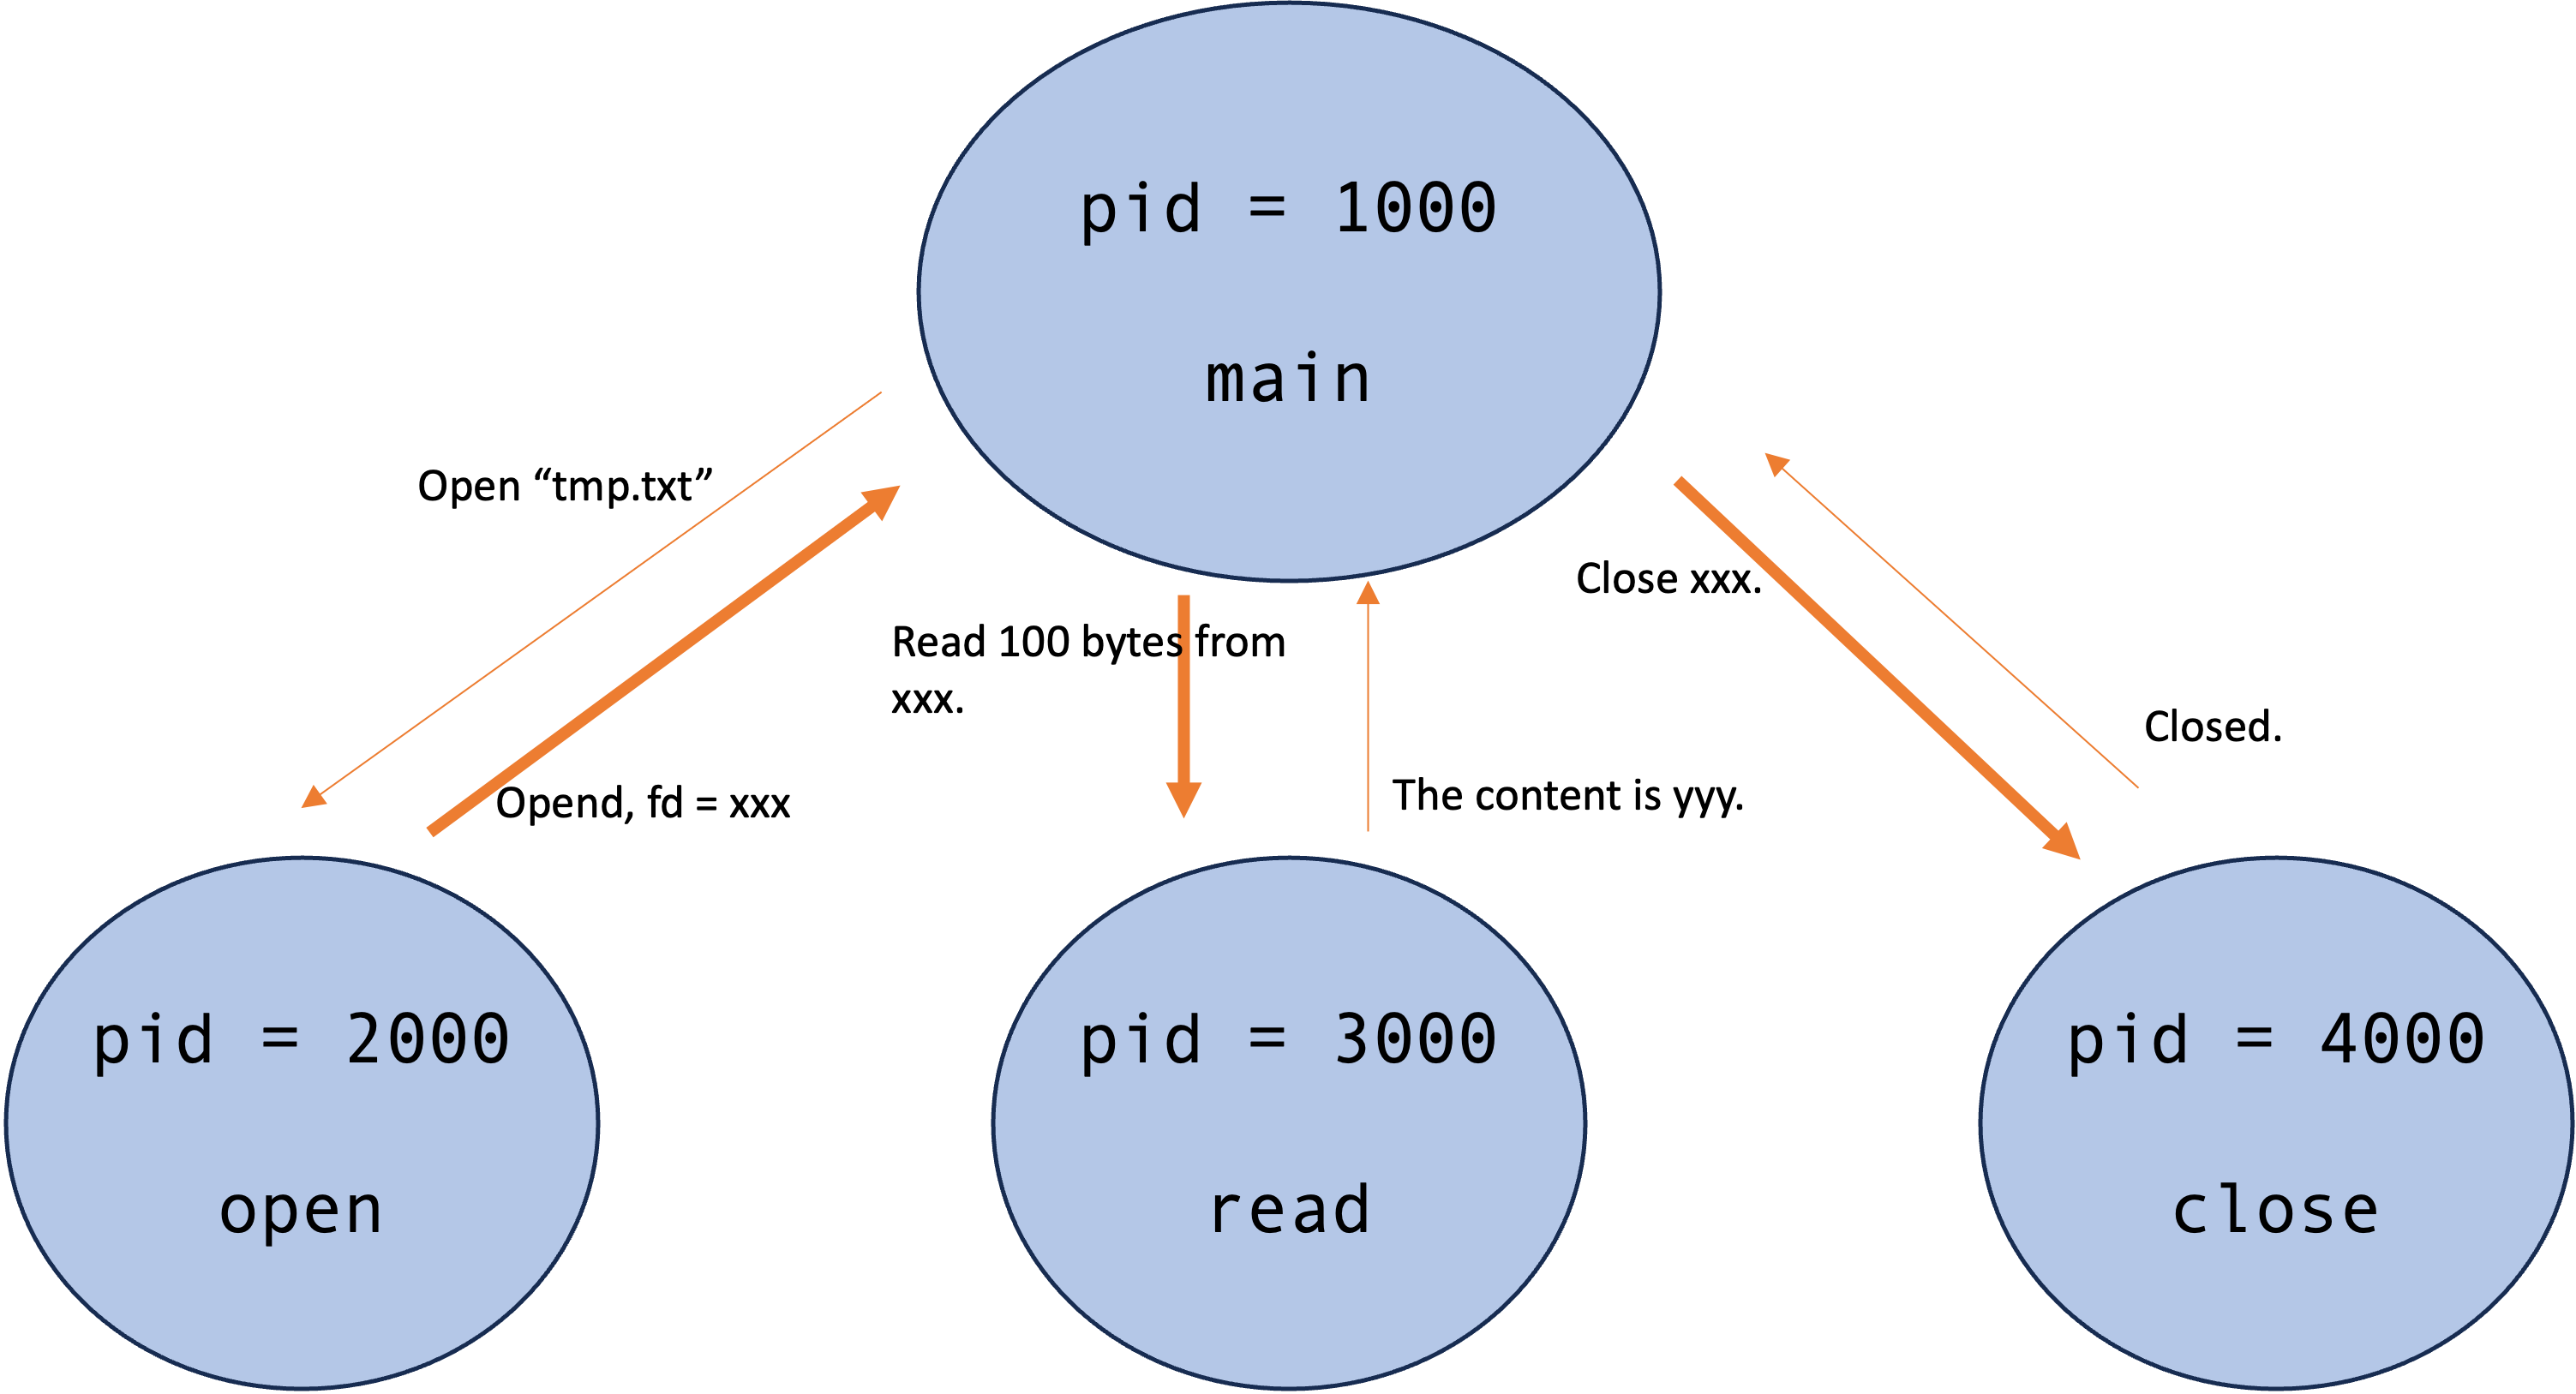
\includegraphics[width=1.8\columnwidth]{./img/fd_transfer.png}
  \end{center}
  \caption{fff}
  \label{img:fd-transfer}
\end{figure*}
"But I must explain to you how all this mistaken idea of denouncing pleasure and praising pain was born and I will give you a complete account of the system, and expound the actual teachings of the great explorer of the truth, the master-builder of human happiness. No one rejects, dislikes, or avoids pleasure itself, because it is pleasure, but because those who do not know how to pursue pleasure rationally encounter consequences that are extremely painful. Nor again is there anyone who loves or pursues or desires to obtain pain of itself, because it is pain, but because occasionally circumstances occur in which toil and pain can procure him some great pleasure. To take a trivial example, which of us ever undertakes laborious physical exercise, except to obtain some advantage from it? But who has any right to find fault with a man who chooses to enjoy a pleasure that has no annoying consequences, or one who avoids a pain that produces no resultant pleasure?"
